\chapter{指针}

\section{指针}

\subsection{指针(Pointer)}

每个变量都会在内存中占用一定的空间,不同类型的变量占用的空间大小也不同。每个空间都有一个地址,一般采用十六进制表示,如0x0060FEFC。\\

有时候需要通过变量的地址对变量进行操作,这时候就需要将变量的地址保存起来,保存地址的变量就成为指针。

\begin{figure}[H]
    \centering
    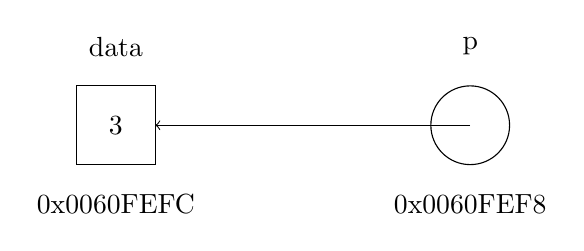
\begin{tikzpicture}
        \draw (0,0) rectangle node{3} (1,1);
        \draw (0.5,1.5) node{data};
        \draw (0.5,-0.5) node{0x0060FEFC};

        \draw (5,0.5) circle (0.5);
        \draw (5,1.5) node{p};
        \draw (5,-0.5) node{0x0060FEF8};

        \draw[->] (5,0.5) -- (1,0.5);
    \end{tikzpicture}
\end{figure}

*用于声明一个指针变量,例如int *p表示p是一个指针,指向一个int类型的变量的地址。通过取地址运算符\&可以获取变量的地址,占位符\%p能够以十六进制的形式输出地址。\\

既然指针保存了另一个变量的地址,那么通过指针就可以访问到那个变量上的数据。在指针变量前使用*运算符,就可以获取到指针所指向的变量的值。

\begin{figure}[H]
    \centering
    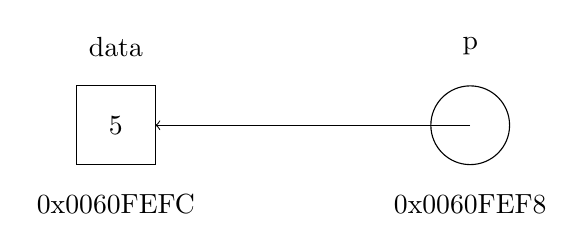
\begin{tikzpicture}
        \draw (0,0) rectangle node{5} (1,1);
        \draw (0.5,1.5) node{data};
        \draw (0.5,-0.5) node{0x0060FEFC};

        \draw (5,0.5) circle (0.5);
        \draw (5,1.5) node{p};
        \draw (5,-0.5) node{0x0060FEF8};

        \draw[->] (5,0.5) -- (1,0.5);
    \end{tikzpicture}
\end{figure}

\mybox{指针}

\begin{lstlisting}[language=C]
#include <stdio.h>

int main() {
    int data = 3;
    int *p = &data;

    printf("Value of data: %d\n", data);
    printf("Address of data: %p\n", &data);
    
    printf("Value of p: %p\n", p);
    printf("Address of p: %p\n", &p);
    printf("Value of data pointed by p: %d\n", *p);
    
    *p = 5;

    printf("Value of data: %d\n", data);
    printf("Value of data pointed by p: %d\n", *p);

    return 0;
}
\end{lstlisting}

\begin{tcolorbox}
    \mybox{运行结果}
    \begin{verbatim}
Value of data: 3
Address of data: 000000000061FE1C
Value of p: 000000000061FE1C     
Address of p: 000000000061FE10   
Value of data pointed by p: 3
Value of data: 5
Value of data pointed by p: 5
	\end{verbatim}
\end{tcolorbox}

为什么不直接修改变量的值,还要多此一举通过指针修改呢?\\

例如需要实现swap()用于交换两个变量的值,由于传递参数是按值传递(pass by value),所以交换的仅仅只是swap()中局部变量的值。\\

这种情况下就需要使用指针,将需要交换的变量的地址传递给swap(),然后在swap()中交换这两个地址上的值。\\

\mybox{交换}

\begin{lstlisting}[language=C]
#include <stdio.h>

void swap(int *data1, int *data2) {
    int temp = *data1;
    *data1 = *data2;
    *data2 = temp;
}

int main() {
    int a = 3;
    int b = 5;

    printf("Before: a = %d, b = %d\n", a, b);
    swap(&a, &b);
    printf("After: a = %d, b = %d\n", a, b);
    return 0;
}
\end{lstlisting}

\begin{tcolorbox}
    \mybox{运行结果}
    \begin{verbatim}
Before: a = 3, b = 5
After: a = 5, b = 3
	\end{verbatim}
\end{tcolorbox}

函数最多只能返回一个值,但如果需要有多个值需要返回,就可以使用指针将数据带回。\\

\mybox{一元二次方程}

\begin{lstlisting}[language=C]
#include <stdio.h>
#include <stdbool.h>
#include <math.h>

/**
 * Solve quadratic equation ax^2 + bx + c = 0.
 * @param a coefficient of x^2
 * @param b coefficient of x
 * @param c constant
 * @param x1 pointer to the first root
 * @param x2 pointer to the second root
 * @return true if the equation has real roots, false otherwise.
 */
bool solver(double a, double b, double c, double *x1, double *x2) {
    double delta = b * b - 4 * a * c;
    if (delta < 0) {
        return false;
    }
    *x1 = (-b + sqrt(delta)) / (2 * a);
    *x2 = (-b - sqrt(delta)) / (2 * a);
    return true;
}

int main() {
    double a, b, c;
    double x1, x2;

    printf("Quadratic equation ax^2 + bx + c = 0\n");
    printf("Enter coefficients a, b, c: ");
    scanf("%lf%lf%lf", &a, &b, &c);

    if (solver(a, b, c, &x1, &x2)) {
        printf("x1 = %.2f, x2 = %.2f\n", x1, x2);
    } else {
        printf("No real roots\n");
    }

    return 0;
}
\end{lstlisting}

\begin{tcolorbox}
    \mybox{运行结果}
    \begin{verbatim}
Quadratic equation ax^2 + bx + c = 0
Enter coefficients a, b, c: 1 -9 20
x1 = 5.00, x2 = 4.00
	\end{verbatim}
\end{tcolorbox}

\vspace{0.5cm}

\subsection{NULL}

如果一个变量声明时没有初始化,那么它的值是不确定的。声明指针时如果不对指针进行初始化,那么它就会指向一块不确定的内存地址,这种指针被称为野指针。\\

使用野指针可能会导致程序崩溃,因为它可能指向一个不可访问的内存地址。因此,如果指针没有指向一个确定的内存地址时,应该将其赋值为空指针NULL。

\vspace{-0.5cm}

\begin{lstlisting}[language=C]
int *p = NULL;
\end{lstlisting}

\newpage

\section{指针与数组}

\subsection{指针与数组}

数组名本质上就是一个指针,它指向数组的首地址。因此在获取数组的地址时,可以不使用\&运算符。\\

\begin{figure}[H]
    \centering
    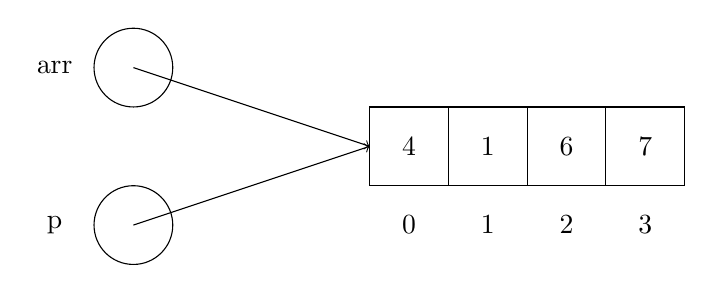
\begin{tikzpicture}
        \draw (0,1) circle (0.5);
        \draw (-1,1) node{arr};

        \draw (0,-1) circle (0.5);
        \draw (-1,-1) node{p};

        \draw (3,-0.5) rectangle (7,0.5);
        \draw (4,-0.5) -- (4,0.5);
        \draw (5,-0.5) -- (5,0.5);
        \draw (6,-0.5) -- (6,0.5);

        \draw (3.5,0) node {4};
        \draw (4.5,0) node {1};
        \draw (5.5,0) node {6};
        \draw (6.5,0) node {7};

        \draw (3.5,-1) node {0};
        \draw (4.5,-1) node {1};
        \draw (5.5,-1) node {2};
        \draw (6.5,-1) node {3};

        \draw[->] (0,1) -- (3,0);
        \draw[->] (0,-1) -- (3,0);
    \end{tikzpicture}
\end{figure}

当对一个指向数组的指针进行加减运算时(如p++和p--),并不是将地址加1或减1,而是根据指针的类型加或减对应字节的长度。例如p是一个int型指针,那么p++会将地址加4(int占4个字节)、p -= 2会将地址减8。\\

\mybox{指针与数组}

\begin{lstlisting}[language=C]
#include <stdio.h>

int main() {
    int arr[] = {4, 1, 6, 7};
    int n = sizeof(arr) / sizeof(arr[0]);
    int *p = arr;

    printf("Address of arr: %p\n", arr);
    for (int i = 0; i < n; i++) {
        printf("Address of arr[%d]: %p\n", i, &arr[i]);
    }

    printf("Value of p: %p\n", p);
    for (int i = 1; i < n; i++) {
        printf("Value of p + %d: %p\n", i, p + i);
    }

    *p = 9;
    *(p + 1) = 8;
    *(p + 2) = 7;
    *(p + 3) = 6;

    for (int i = 0; i < n; i++) {
        printf("arr[%d]: %d\n", i, arr[i]);
    }

    return 0;
}
\end{lstlisting}

\begin{tcolorbox}
    \mybox{运行结果}
    \begin{verbatim}
Address of arr: 000000000061FDF0
Address of arr[0]: 000000000061FDF0
Address of arr[1]: 000000000061FDF4
Address of arr[2]: 000000000061FDF8
Address of arr[3]: 000000000061FDFC
Value of p: 000000000061FDF0
Value of p + 1: 000000000061FDF4
Value of p + 2: 000000000061FDF8
Value of p + 3: 000000000061FDFC
arr[0]: 9
arr[1]: 8
arr[2]: 7
arr[3]: 6
	\end{verbatim}
\end{tcolorbox}

\vspace{0.5cm}

\subsection{数组与函数}

数组作为函数参数时,会将数组的地址传递给函数,函数接收到的是一个指向数组首地址的指针。由于在函数中失去了数组长度的信息,并不能通过sizeof()计算出数组的长度(计算得到的是一个指针变量所占的空间),因此将数组传入函数时,还需要将其长度一并作为参数传给函数。\\

\mybox{查找}

\begin{lstlisting}[language=C]
#include <stdio.h>

int search(int *arr, int n, int key) {
    for (int i = 0; i < n; i++) {
        if (arr[i] == key) {
            return i;
        }
    }
    return -1;
}

int main() {
    int arr[] = {4, 7, 1, 3, 9, 2};
    int n = sizeof(arr) / sizeof(arr[0]);

    int index = search(arr, n, 3);
    if (index == -1) {
        printf("Not found\n");
    } else {
        printf("Found at index %d\n", index);
    }

    return 0;
}
\end{lstlisting}

\begin{tcolorbox}
    \mybox{运行结果}
    \begin{verbatim}
Found at index 3
	\end{verbatim}
\end{tcolorbox}

\newpage

\section{指针与字符串}

\subsection{指针与字符串}

数组和指针都可以用于定义一个字符串,但是它们内存分配的方式不同,从而导致它们的使用方式也不同。\\

以数组形式定义的字符串,每个字符保存在一个字符数组中。这样的字符串是可以修改的,与普通的数组类似。\\

但是如果让一个指针指向一个字符串,那么这个字符串会被存储在常量区。常量区中的数据是不可以修改的,因此使用指针去修改字符串会导致程序崩溃。\\

\begin{figure}[H]
    \centering
    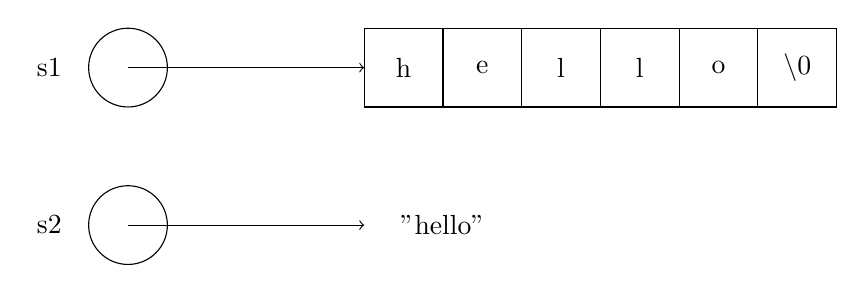
\begin{tikzpicture}
        \draw (0,0) circle (0.5);
        \draw (-1,0) node{s1};

        \draw (3,-0.5) rectangle (9,0.5);
        \draw (4,-0.5) -- (4,0.5);
        \draw (5,-0.5) -- (5,0.5);
        \draw (6,-0.5) -- (6,0.5);
        \draw (7,-0.5) -- (7,0.5);
        \draw (8,-0.5) -- (8,0.5);

        \draw (3.5,0) node {h};
        \draw (4.5,0) node {e};
        \draw (5.5,0) node {l};
        \draw (6.5,0) node {l};
        \draw (7.5,0) node {o};
        \draw (8.5,0) node {$ \backslash $0};

        \draw[->] (0,0) -- (3,0);

        \draw (0,-2) circle (0.5);
        \draw (-1,-2) node{s2};
        \draw (4,-2) node {"hello"};
        \draw[->] (0,-2) -- (3,-2);
    \end{tikzpicture}
\end{figure}

\vspace{-0.5cm}

\begin{lstlisting}[language=C]
char s1[] = "hello";
s1[0] = 'H';
printf("s1 = %s\n", s1);

char *s2 = "hello";
s2[0] = 'H';        // error
printf("s2 = %s\n", s2);
\end{lstlisting}

在对指向字符串的指针进行赋值操作的时候,并不会产生新的字符串,只是让两个指针都指向同一个字符串,对任意一个指针做的操作都会影响另一个指针。\\

\begin{figure}[H]
    \centering
    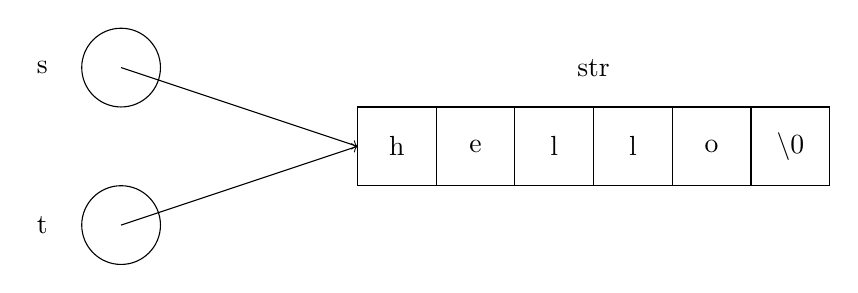
\begin{tikzpicture}
        \draw (0,1) circle (0.5);
        \draw (-1,1) node{s};

        \draw (0,-1) circle (0.5);
        \draw (-1,-1) node{t};

        \draw (3,-0.5) rectangle (9,0.5);
        \draw (4,-0.5) -- (4,0.5);
        \draw (5,-0.5) -- (5,0.5);
        \draw (6,-0.5) -- (6,0.5);
        \draw (7,-0.5) -- (7,0.5);
        \draw (8,-0.5) -- (8,0.5);

        \draw (3.5,0) node {h};
        \draw (4.5,0) node {e};
        \draw (5.5,0) node {l};
        \draw (6.5,0) node {l};
        \draw (7.5,0) node {o};
        \draw (8.5,0) node {$ \backslash $0};
        \draw (6,1) node {str};

        \draw[->] (0,1) -- (3,0);
        \draw[->] (0,-1) -- (3,0);
    \end{tikzpicture}
\end{figure}

\mybox{指向字符串的指针}

\begin{lstlisting}[language=C]
#include <stdio.h>

int main() {
    char str[] = "hello";
    char *s = str;
    char *t = s;

    s[0] = 'H';
    printf("s = %s\n", s);
    printf("t = %s\n", t);

    return 0;
}
\end{lstlisting}

\begin{tcolorbox}
    \mybox{运行结果}
    \begin{verbatim}
s = Hello
t = Hello
	\end{verbatim}
\end{tcolorbox}

\vspace{0.5cm}

\subsection{指针与二维数组}

\newpage

\section{动态内存申请}

\subsection{malloc()}

C99支持声明数组时使用变量作为数组的大小。

\vspace{-0.5cm}

\begin{lstlisting}[language=C]
int n = 50;
int arr[n];
\end{lstlisting}

但是在C99之前的版本中,需要使用动态内存申请的方式进行数组空间的开辟。malloc()的功能是向系统申请指定的内存空间(以字节为单位),使用该函数需要包含头文件stdlib.h。\\

malloc()函数原型为:

\vspace{-0.5cm}

\begin{lstlisting}[language=C]
void* malloc(size_t size);
\end{lstlisting}

malloc()的返回值为void *类型,表示一个指向申请到的空间的首地址,是一个无类型的指针,开发者需要自行转换为自己需要的类型。如果malloc()申请内存失败,则会返回空指针NULL。\\

\mybox{耗尽所有可申请到的内存空间}

\begin{lstlisting}[language=C]
#include <stdio.h>
#include <stdlib.h>

int main() {
    void *p;
    int cnt = 0;

    // 每次申请100MB的空间
    while((p = malloc(100 * 1024 * 1024))) {
        cnt++;
    }
    printf("一共分配了%dMB空间\n", cnt*100);
    return 0;
}
\end{lstlisting}

\begin{tcolorbox}
    \mybox{运行结果}
    \begin{verbatim}
一共分配了1900MB空间
	\end{verbatim}
\end{tcolorbox}

通过malloc()申请来的空间是需要归还给操作系统的,否则程序长时间运行内存会逐渐下降。\\

通过free()可以把申请来的空间释放,但是有两点需要注意:

\begin{enumerate}
    \item 只能释放通过malloc()申请得到的空间。
    \item 只能通过空间的首地址进行释放。
\end{enumerate}

\vspace{0.5cm}

\mybox{动态申请内存空间}

\begin{lstlisting}[language=C]
#include <stdio.h>
#include <stdlib.h>

int main() {
    int n;
    printf("班级人数:");
    scanf("%d", &n);

    int *scores = (int *)malloc(sizeof(int) * n);
    if(!scores) {
        fprintf(stderr, "内存申请失败\n");
        exit(1);
    }

    int total = 0;
    for(int i = 0; i < n; i++) {
        printf("第%d个学生成绩:", i+1);
        scanf("%d", &scores[i]);
        total += scores[i];
    }

    printf("平均分:%.2f\n", 1.0 * total / n);
    free(scores);
    return 0;
}
\end{lstlisting}

\begin{tcolorbox}
    \mybox{运行结果}
    \begin{verbatim}
班级人数:5
第1个学生成绩:67
第2个学生成绩:98
第3个学生成绩:100
第4个学生成绩:53
第5个学生成绩:65
平均分:76.60
	\end{verbatim}
\end{tcolorbox}

在函数中的定义的字符数组是局部变量,其作用域和生命周期仅在函数内有效,如果将其作为函数返回值返回,在函数外部无法访问到该变量的内容。\\

\mybox{函数返回字符串(Bug版本)}

\begin{lstlisting}[language=C]
#include <stdio.h>
#include <stdlib.h>
#include <string.h>

/**
    * @brief  生成一段自我介绍
    * @param  name: 姓名
    * @param  age: 年龄
    * @retval 指定格式字符串:大家好,我叫{name},今年{age}岁。
    */
char* generateInfo(char *name, int age) {
    char info[128] = "大家好,我叫";
    char age_str[8] = "";
    strcat(info, name);
    strcat(info, ",今年");
    // itoa()函数用于将整数转为字符串
    // 把age以10进制转换为字符串保存到age_str
    strcat(info, itoa(age, age_str, 10));
    strcat(info, "岁。");
    return info;
}

int main() {
    printf("%s\n", generateInfo("极夜酱", 17));
    return 0;
}
\end{lstlisting}

\begin{tcolorbox}
    \mybox{运行结果}
    \begin{verbatim}
warning:
function returns address of local variable [-Wreturn-local-addr]
	\end{verbatim}
\end{tcolorbox}

\vspace{0.5cm}

\mybox{函数返回字符串(正确版本)}

\begin{lstlisting}[language=C]
#include <stdio.h>
#include <stdlib.h>
#include <string.h>

/**
    * @brief  生成一段自我介绍
    * @param  name: 姓名
    * @param  age: 年龄
    * @retval 指定格式字符串:大家好,我叫{name},今年{age}岁。
    */
char* generateInfo(char *name, int age) {
    char *info = (char *)malloc(sizeof(char) * 128);
    if(!info) {
        return NULL;
    }
    char age_str[8] = "";
    strcpy(info, "大家好,我叫");
    strcat(info, name);
    strcat(info, ",今年");
    // itoa()函数用于将整数转为字符串
    // 把age以10进制转换为字符串保存到age_str
    strcat(info, itoa(age, age_str, 10));
    strcat(info, "岁。");
    return info;
}

int main() {
    printf("%s\n", generateInfo("极夜酱", 17));
    return 0;
}
\end{lstlisting}

\begin{tcolorbox}
    \mybox{运行结果}
    \begin{verbatim}
大家好,我叫极夜酱,今年17岁。
	\end{verbatim}
\end{tcolorbox}

\vspace{0.5cm}

\subsection{内存管理}

内存通常包括了栈区(stack)、堆区(heap)、数据区、程序代码区:

\begin{itemize}
    \item 栈区:由编译器自动分配和释放,存放函数的参数值、局部变量的值等。

    \item 堆区:一般由程序员分配和释放,若程序员不释放,程序结束后被OS回收。

    \item 数据区:存放全局变量和静态变量,程序结束后由系统释放。

    \item 程序代码区:存放函数体的二进制代码。
\end{itemize}

\begin{figure}[H]
    \centering
    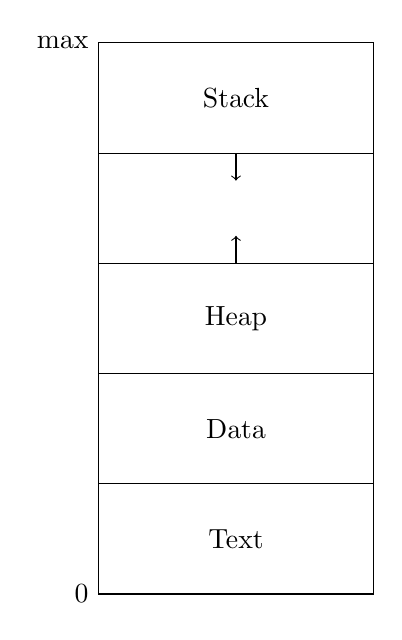
\begin{tikzpicture}[scale=0.7]
        \draw[-] (0,0) -- (0,10) -- (5,10) -- (5,0) -- (0,0);
        \draw[-] (0,2) -- (5,2);
        \draw[-] (0,4) -- (5,4);
        \draw[-] (0,6) -- (5,6);
        \draw[-] (0,8) -- (5,8);

        \draw (0,0) node[left] {0};
        \draw (0,10) node[left] {max};

        \draw (2.5,1) node {Text};
        \draw (2.5,3) node {Data};
        \draw (2.5,5) node {Heap};
        \draw (2.5,9) node {Stack};

        \draw[->] (2.5,8) -- (2.5,7.5);
        \draw[->] (2.5,6) -- (2.5,6.5);
    \end{tikzpicture}
    \caption{内存管理}
\end{figure}

\newpage